%%%% Proceedings format for most of ACM conferences (with the exceptions listed below) and all ICPS volumes.
\documentclass[sigconf]{acmart}
%%%% As of March 2017, [siggraph] is no longer used. Please use sigconf (above) for SIGGRAPH conferences.

%%%% Proceedings format for SIGPLAN conferences 
% \documentclass[sigplan, anonymous, review]{acmart}

%%%% Proceedings format for SIGCHI conferences
% \documentclass[sigchi, review]{acmart}

%%%% To use the SIGCHI extended abstract template, please visit
% https://www.overleaf.com/read/zzzfqvkmrfzn

\begin{document}

\title{Higher-order networks: A survey of analysis methods for sequential network data}

% The "author" command and its associated commands are used to define the authors and their affiliations.
\author{Bradley Dice}
\email{bdice@bradleydice.com}
\orcid{0000-0002-9983-0770}
\affiliation{
  \institution{University of Michigan \\ Department of Physics}
  \city{Ann Arbor}
  \state{Michigan}
  \postcode{48109}
}

\author{Daniel McCusker}
\email{dmccuske@umich.edu}
\affiliation{
  \institution{University of Michigan \\ Applied Physics}
  \city{Ann Arbor}
  \state{Michigan}
  \postcode{48109}
}

\author{Shannon Moran}
\email{moranse@umich.edu}
\orcid{0000-0002-3579-3149}
\affiliation{
 \institution{University of Michigan \\ Department of Chemical Engineering}
  \city{Ann Arbor}
  \state{Michigan}
  \postcode{48109}
 }

\renewcommand{\shortauthors}{Dice, et al.}

% The abstract is a short summary of the work to be presented in the article.
% \begin{abstract}
% \end{abstract}

% Keywords, separate with commas.
\keywords{higher order networks, graph mining, network dynamics, map equation, Markov processes}

% \begin{teaserfigure}[b]
%   \centering
%   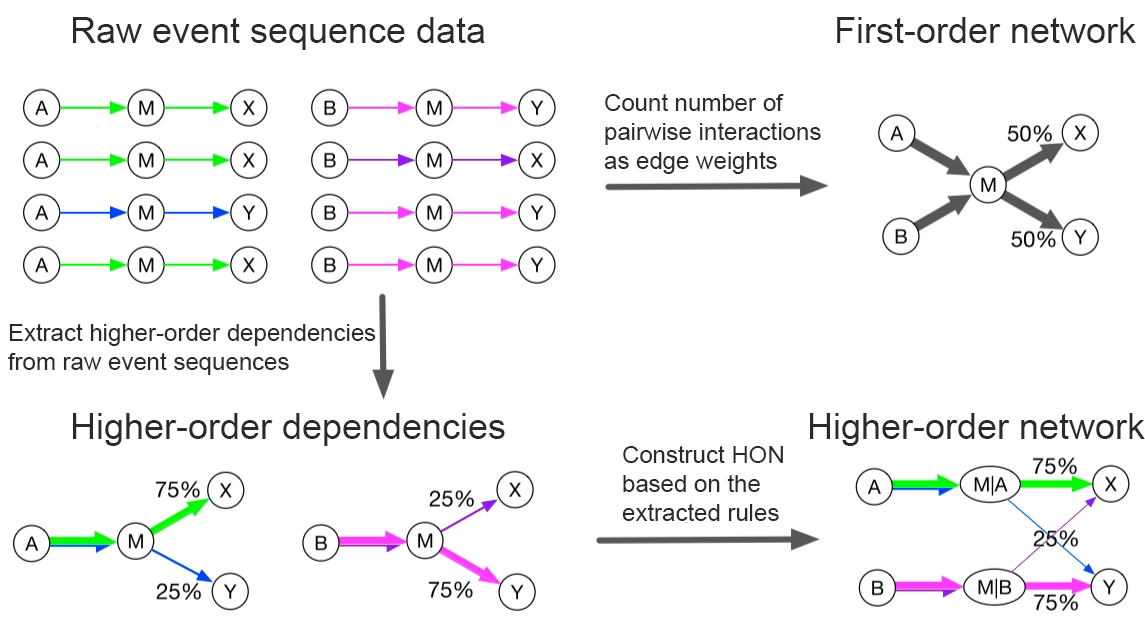
\includegraphics[width=0.7\textwidth]{HON.png}
%   \caption{Higher-order networks, visualized. source: http://www.higherordernetwork.com/}
%   \label{fig:HON}
% \end{teaserfigure}

% Show author, affiliation, and title information
\maketitle

\section{Introduction}
Traditional representations of networks fail to capture higher-order correlations, such as the journey a ship may take between multiple ports. This understanding is important for predicting network dynamics more than one step into the future, as well as capturing the proper roles of nodes and their communities in a network.

We are looking to survey and implement \textbf{higher-order network analysis on flow/routing data}. In our survey of the literature, we are looking to understand the state-of-the-art in this field.

\section{Topic selection}

We initially sought a recent academic paper to replicate and build upon. As a group, we realized we had three core decisions to make for our proposal topic.

(1) \textbf{Prediction or analysis?} Many recent academic papers are interested in analyzing graphs with the goal of predicting linkages, structures, etc. There is also rich literature on transforming and analyzing graphs. We've decided to focus on \textbf{graph analysis} (e.g. centralities, cluster idenfication), with a potential extension to prediction only if time allows. 

(2) \textbf{Choice of network structure (leading to choice of data set).} As a group, we are interested in analyzing a business-driven data set; in particular, routing data for freight or transportation traffic. This led us to investigate methods for encoding and analyzing such data on graphs while preserving the relative traffic through given nodes. Higher-order networks (HONs) have been used to represent such data \cite{Xu2016, Rosvall2014, Edler2017, Benson2016, Benson2018}. Additionally, analysis of these graph structures is an active area of research. Some approaches such as aggregate flow networks have been used for sequential data \cite{Safavi2018}, which could be helpful in a coarse-grained, ``macroeconomic'' sense. However, we are interested in finer details such as pathways and trajectories. We will decide on the specific data set to use when finalizing our project proposal.

(3) \textbf{Methods to use.} Here, our first survey of the literature sought to understand what methods are currently used in analyzing HONs. We began with literature recommended in the course materials (in the ``further reading'' sections), then expanded our search to related papers. 

One advantage and challenge of this area is that many of the relevant works in also publish their code and use publicly available data sources. (Of course, this does not mean that it is straight-forward to replicate the results -- just that there is code to do so!) Consequently, our project won't just be replicating a paper, but rather extending and combining the methods from several papers.

\section{Distribution of work}
Each group member (Bradley, Dan, and Shannon) was responsible for writing up two paper summaries. All group members agreed unanimously on the topic and contributed equally to selecting relevant papers and writing the survey. %Moving forward, we will have more defined modules on the project.

% Technical relevance section
\section{Methods discussed in summary}
%How do these papers relate to each other? Are they solving a new problem or improving an existing method? What are the main techniques they are using?

Two common techniques are MapEquation and Infomap. The MapEquation software implements the Infomap optimization algorithm for community detection, and is based on the ``map equation,'' an information-theoretic tool based on flows on networks. Infomap can perform community detection routines on directed, undirected, weighted, unweighted, multi-level and higher-order Markov networks (``memory networks''). Infomap reveals levels of network structure that are not apparent when considering only first-order flow processes, so it improves on existing community detection routines but is not solving a new problem \textit{per se}.

We can represent networks with both topological and dynamic data as ``HON'' (higher-order networks). We highlight two approaches available for transforming first-order networks to representations that preserve flow trajectory information \cite{Xu2016,Scholtes2017}.


\section{Survey: Graph representation}

\subsection{``Representing higher-order dependencies in networks'' \cite{Xu2016}} \label{paper:HON}
Higher-order dependencies (sometimes called ``memory'') in networks formed from sequential data are critical for proper clustering, predicting future edge traversals, and rankings of nodes.
This paper introduces the (confusingly-named) ``HON'' algorithm for converting a network of nodes and edges into a new representation with split nodes that represent the common paths taken to get to that node.
For an input of any network of sequential data, a rule-based extraction is performed to produce a unique graph that includes dependencies up to a specified maximum order.
Past work in this field has used fixed-order representations, typically of order 1 or 2, but the HON method detects when higher-order dependencies are present and adds them in a way that maximizes sparsity where possible, capturing only higher order nodes that play a significant role (which many previous papers have neglected due to the explosive state space of possible paths over nodes).
Some strengths of this method are its uniqueness and sparsity - it is much more efficient than fixed-order networks and is less likely to detect spurious high-order correlations because of its tests for ``significance.''
However, its utility is restricted to sequence-like data in discretized time.
Thus, continuous-time data must be adapted into a discrete sequence for use.
Moreover, methods like HON are ``windowed;'' they cannot distinguish changes in network dynamics over the course of their observations.
Separate networks must be built from different portions of the time series in order to distinguish changes in the network flows over time.
Lastly, diffusion processes on networks are inherently first-order, so HON cannot provide any advantages for understanding problems such as those faced in epidemiology, where diffusion models the spread of disease.
Of the 14 papers on Web of Science that cite this work, many of their references are only to mention that ``higher-order'' concepts exist, and it seems that few authors have actually read the paper (the context doesn't match the cited content) or used its methods directly (though the code is freely available!).

\subsection{``When is a network a network?'' \cite{Scholtes2017}} \label{paper:wianan}
While first-order networks are sufficient for capturing the topology and frequency of data, they lose the memory of trajectory histories in the underlying events. This paper's innovation is a framework that uses statistical analysis to determine the number of layers $k$ needed to capture the temporal effects in a network with multiple correlation lengths. We find the authors' demonstration of the importance of accounting for autocorrelations in analysis (using the example of PageRank) compelling. 
However, it's not clear from our survey that this is the best way of developing higher-order representations of network data. The authors only compare their resulting higher-order Markov chains against baseline Markov order detection techniques, not other HON representations.

Importantly, this paper utilizes five data sets that we can consider for our own project (280k flight itineraries, 4.2M London metro trips, 30k APS scientist career trajectories, 76k Wikipedia click paths, and 1M click streams on MSNBC).

\subsection{``Simplicial closure and higher-order link prediction'' \cite{Benson2018}}
Another way to study dynamics on networks involves generalization from pairwise interactions (``dyadic'' edges) to $k$-way interactions (simplices that are $k$-cliques). This paper discusses how data on groupings of nodes over time (e.g. paper coauthorships or tags on forum posts) can be used for link prediction. Unsurprisingly, prediction accuracy goes up when considering the 3-way and 4-way connections that occur in the data. This paper mentions HON \cite{Xu2016}, but does not show direct comparisons. The edge predictions from this method are more aware of local structure, because triangles and higher-order simplices capture a better understanding of nodes' environments -- the information about simplicial closure is valuable for accurately predicting new edges. However, the additional computational cost of this higher-order analysis may not be necessary if dyadic (pairwise) models are sufficient. Moreover, this method is less relevant unless the predictions of interest are themselves sets or $k$-cliques (e.g. who will coauthor together?).

\section{Survey: Analyzing Higher-Order Networks}

\subsection{``Higher-order organization of complex networks'' \cite{Benson2016}} \label{paper:HONorganization}
This paper's key innovation is a method for identifying the most optimal clusters in a higher-order network.
As we have found during this literature survey, both developing optimal higher-order representations for data (e.g. \cite{Scholtes2017}) and analyzing that data are non-trivial.
The authors develop an extension of spectral graph clustering to account for higher-order structures in networks.
For a given topological motif $M$ (several examples are provided in the paper), the algorithm looks for nodes $S$ that minimize ``cutting'' instances of $M$ while also participating in many instances of $M$.
% They define this as a ``motif conductance'' they seek to minimize as $\phi_M(S) = \text{cut}_M(S,\bar{S})/\text{min}[\text{vol}_M(S),\text{vol}_M(\bar{S})]$, where where $\bar{S}$ denotes the remainder of the nodes $\text{cut}(S,\bar{S})$ is the number of instances of motif $M$ with at least one node in $\bar{S}$ and one in $S$, and $\text{vol}_M(S)$ is the number of nodes in instances of $M$ that reside in $S$.

Detailed supplemental information describe the implementation of the algorithms, with several computational strengths. The algorithm is easily parallelized, and is able to find a very-nearly optimal solution with some clever short-cuts to find near-optimal sets of $S$. As a result, this algorithm is easily scalable (the authors assert up to ``billions of edges''). Additionally, this algorithm supports directed, undirected, and weighted graphs.

Our hesitation with this work is that it relies upon domain knowledge to suggest a motif of interest. While the supplemental information suggests that this algorithm can also be used to find motifs to explore, that is not this work's primary focus.

\subsection{``Memory in network flows'' \cite{Rosvall2014}} \label{paper:memory}
This paper illustrates the importance of second-order Markov effects for processes happening on networks. It analyzes random walks on various graphs using MapEquation and InfoMap, and demonstrates significant second-order effects for community detection, ranking, and information spreading. The paper shows these structural effects on several data sets, including airline traffic, journal citations, hospital patients, and email messages. A weakness of the paper is that it required more available data, which may not always be available for networks of interest. The method is also limited in that it only studies network flows to second order; as noted in \cite{Xu2016}, some effects are not apparent until considering fifth-order flows, though this will depend on the data set of interest.

\subsection{``Mapping higher-order network flows'' with InfoMap \cite{Edler2017}} \label{paper:infomap}
In this paper, the authors also use Infomap to analyze structure in higher order networks. Specifically, they introduce ``sparse memory networks,'' a network representation that accounts for higher-order Markov dynamics, but also integrates information from multi-layer networks to reduce redundancy in the state nodes. This results in a more compact network structure with abstract representation nodes, and allows for the detection of modular and overlapping communities. However, the paper makes no mention of the ``interpretability'' of these abstract nodes. Moreover, the paper only uses one example data set, and does not illustrate which networks benefit from the improved analysis and which do not. It also doesn't compare the results to a standard community detection routine, so it's hard to intuit the improvement that the paper brings. 

\bibliographystyle{ACM-Reference-Format}
\bibliography{survey}

\appendix
% Any appendix sections would go here

\end{document}
